\subsection{Caso d'uso UC11: Pagina Utente}

\label{UC11}
\begin{figure}
	\centering
	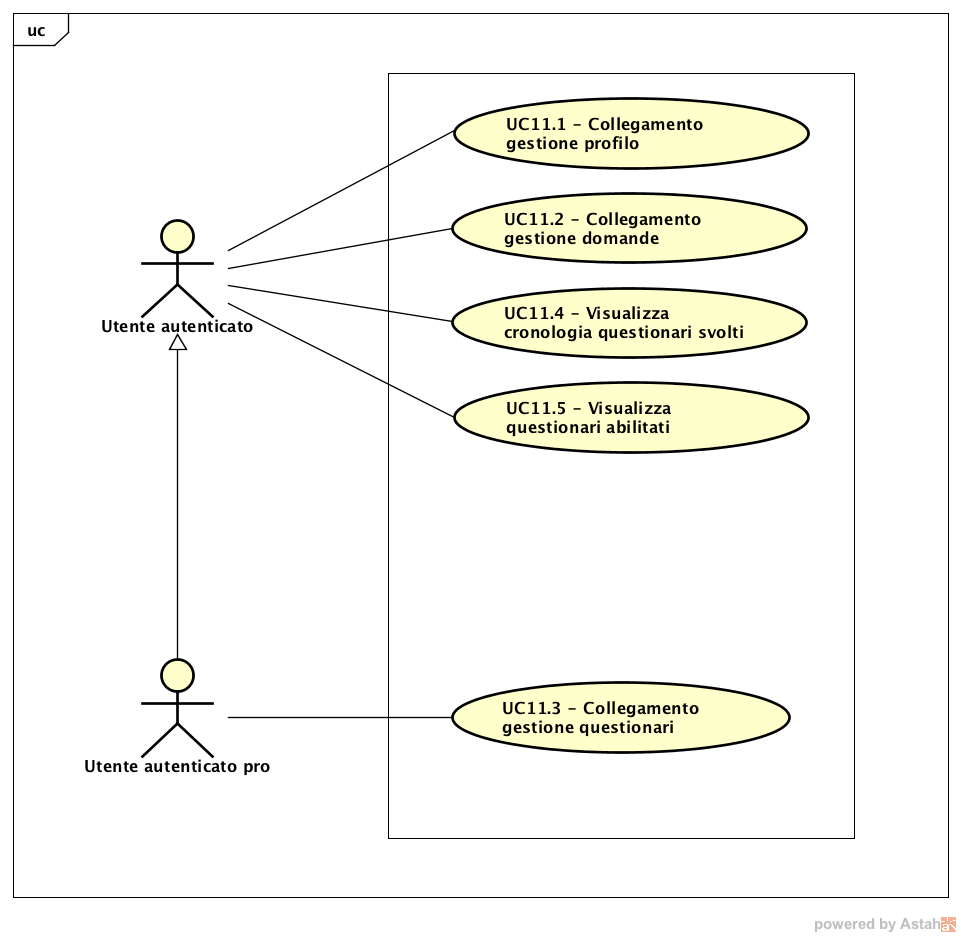
\includegraphics[scale=0.5]{UML/UC11.png}
	\caption{UC11: Gestione pagina utente}
\end{figure}

\begin{itemize}
\item\textbf{Attori}: utente autenticato, utente autenticato pro
\item\textbf{Descrizione}: l'utente da questa pagina può visualizzare tutti i dati del suo profilo, tutte le statistiche dei questionari svolti, può inoltre vedere la cronologia dei questionari svolti, la lista dei questionari da fare e può infine accedere alle varie parti del sistema che gli permettono di modificare il profilo o aggiungere nuove domande e questionari;
\item\textbf{Precondizione}: l'utente è entrato nella pagina di visualizzazione del profilo;
\item\textbf{Postcondizione}: l'utente ha visualizzato i suoi dati;
\item\textbf{Scenario principale}:
\begin{itemize}
\item L'utente ha scelto di andare alla pagina di gestione del profilo (UC11.1);
\item L'utente ha scelto di andare alla pagina di gestione delle domande (UC11.2);  
\item L'utente ha scelto di andare alla pagina di gestione dei questionari (UC11.3).
\end{itemize}
\end{itemize}

\subsubsection{Caso d'uso UC11.1: Collegamento gestione profilo}
\begin{itemize}
\item\textbf{Attori}: utente autenticato, utente autenticato pro
\item\textbf{Descrizione}: l'utente viene portato nella pagina di gestione del profilo dove potrà modificare liberamente tutti i suoi dati;
\item\textbf{Precondizione}: l'utente ha premuto l'apposito link di gestione del profilo;
\item\textbf{Postcondizione}: il sistema ha portato l'utente alla pagina di gestione del profilo;
\item\textbf{Scenario principale}: l'utente si trova nella pagina di gestione del profilo e potrà attuare tutte le modifiche desiderate;
\end{itemize}

\subsubsection{Caso d'uso UC11.2: Collegamento gestione delle domande}
\begin{itemize}
\item\textbf{Attori}: utente autenticato, utente autenticato pro
\item\textbf{Descrizione}: l'utente viene portato nella pagina di gestione delle domande dove potrà inserire o modificare le sue domande;
\item\textbf{Precondizione}: l'utente ha premuto l'apposito link di gestione delle domande;
\item\textbf{Postcondizione}: il sistema ha portato l'utente alla pagina di gestione delle domande;
\item\textbf{Scenario principale}: l'utente si trova nella pagina di gestione delle domande e potrà attuare tutte le modifiche desiderate;
\end{itemize}

\subsubsection{Caso d'uso UC11.1: Collegamento gestione questionari}
\begin{itemize}
\item\textbf{Attori}: utente autenticato, utente autenticato pro
\item\textbf{Descrizione}: l'utente viene portato nella pagina di gestione dei questionari dove potrà compiere tutte le azioni possbili sui questionari;
\item\textbf{Precondizione}: l'utente ha premuto l'apposito link di gestione dei questionari;
\item\textbf{Postcondizione}: il sistema ha portato l'utente alla pagina di gestione dei questionari;
\item\textbf{Scenario principale}: l'utente si trova nella pagina di gestione dei questionari e potrà attuare tutte le modifiche desiderate;
\end{itemize}